\documentclass{article}
\usepackage[utf8]{inputenc}
\usepackage{graphicx}
\usepackage[margin=1in]{geometry}
\usepackage[dvipsnames]{xcolor}
\usepackage{url}
\usepackage{hyperref}
\hypersetup{hidelinks}
\usepackage[numbers]{natbib} % for numeric references
\usepackage{booktabs} % For results table: figure and table will share the top of one page 
\renewcommand{\topfraction}{0.95}
\renewcommand{\textfraction}{0.05}
\setlength{\floatsep}{8pt}
\setlength{\textfloatsep}{10pt}
\setlength{\abovecaptionskip}{4pt}

\begin{document}

\begin{titlepage}
    \begin{center}
        
\includegraphics[width=3cm]{figures/MSP-logo.jpg} 
        \vspace{1cm}
        
        \textbf{\LARGE Reported sleep around the world:}\\
        \textbf{\LARGE Differences by country, age, sex, and commute}
        
        \vspace{1.5cm}
        
        \textbf{\Large Julia Waldmeier (I6341664)}
        
        \vfill
        
        \large Date: \today
        
    \end{center}
\end{titlepage}

\newpage

\section*{Introduction}
%Brief introduction about the topic, phrase the scientific question and place it in a broader context
Adults are advised to sleep at least seven hours per night, and regularly sleeping less is associated with obesity, high blood pressure, cardiovascular disease and higher mortality~\cite{watson}. In this report I ask: in which countries do people report the least sleep, and which groups of people, by age, sex, and length of commute, report the least? 

\section*{Data sample}
%Add here a brief description of the dataset
The data set was collected between May 2016 and July 2017 via the mobile game Sea Hero Quest and published by Coutrot et al.~\cite{coutrot}. It contains 730{,}187 people aged 19 to 70 in 63 countries, with at least 509 people per country. Each player answered the question ``How much sleep do you get on average each night?'' in whole hours from 5 to 10. The file was already cleaned by the authors, so no rows were removed. The 239 people who did not answer the commute question were excluded from the commute comparison only. 

\section*{Data analysis method}
The data analysis was done in R; the figures were made in Python (NumPy, pandas, and Matplotlib). For each group (a country, a sex, an age group or a commute length), I calculated the average reported sleep $\bar{x}$ and its statistical uncertainty $\sigma_{\bar{x}} = s/\sqrt{N}$, where $s$ is the standard deviation and $N$ the number of people in the group. Within each variable, I compared the group with the highest average to the group with the lowest: the difference $\Delta = \bar{x}_a - \bar{x}_b$ has the uncertainty $\sigma_{\Delta} = \sqrt{\sigma_{a}^{2} + \sigma_{b}^{2}}$, since the groups contain different people, and its significance is $|\Delta|/\sigma_{\Delta}$, with $3\sigma$ or more counted as significant. The highest and lowest country were also compared with every other country. Ages were combined into four groups of 13 years each (19--31, 32--44, 45--57, and 58--70). The formula for uncertainty on the difference was checked with the sub-sampling technique (ten random sub-samples): the averages of the two groups are uncorrelated ($|r| \leq 0.10$). Because a large sample makes even a small difference significant, I also give the effect size Hedges' $g = \Delta / s_p$, where $s_p$ is the pooled standard deviation of the individuals in both groups (where 0.2 is small, 0.5 medium, and 0.8 large). To check that one variable does not hide or exaggerate another, every comparison was repeated inside each country, and a multiple linear regression compared people of the same country, sex, age group, and commute. 

\section*{Results and discussion}
% Add here your results, your plots, the discussion about the observation.
Across all respondents the average reported sleep is $7.006 \pm 0.001$~hours, with a standard deviation of 1.06~hours between individuals. Figure~\ref{fig:results} (left) shows the ten countries with the least and the most sleep. Japan is lowest with $6.63 \pm 0.04$~hours and Albania highest with $7.54 \pm 0.04$~hours, a difference of $\Delta = 0.91 \pm 0.06$~hours $=55 \pm 4$~minutes ($16\sigma$). Albania is significantly the highest ($3.9\sigma$ above Slovakia, the second highest), but Japan is not significantly the lowest: eight countries, mostly in Asia and the Middle East, are less than $3\sigma$ from it, so the lowest cannot be identified. Compared with each of these nine countries, Albania reports 45 to 55 minutes more sleep, always $13\sigma$ or more. This is the extreme: the 43 countries in the middle lie within 20 minutes of each other.

\begin{figure}[!t]
\centering
\begin{minipage}[c]{0.34\textwidth}
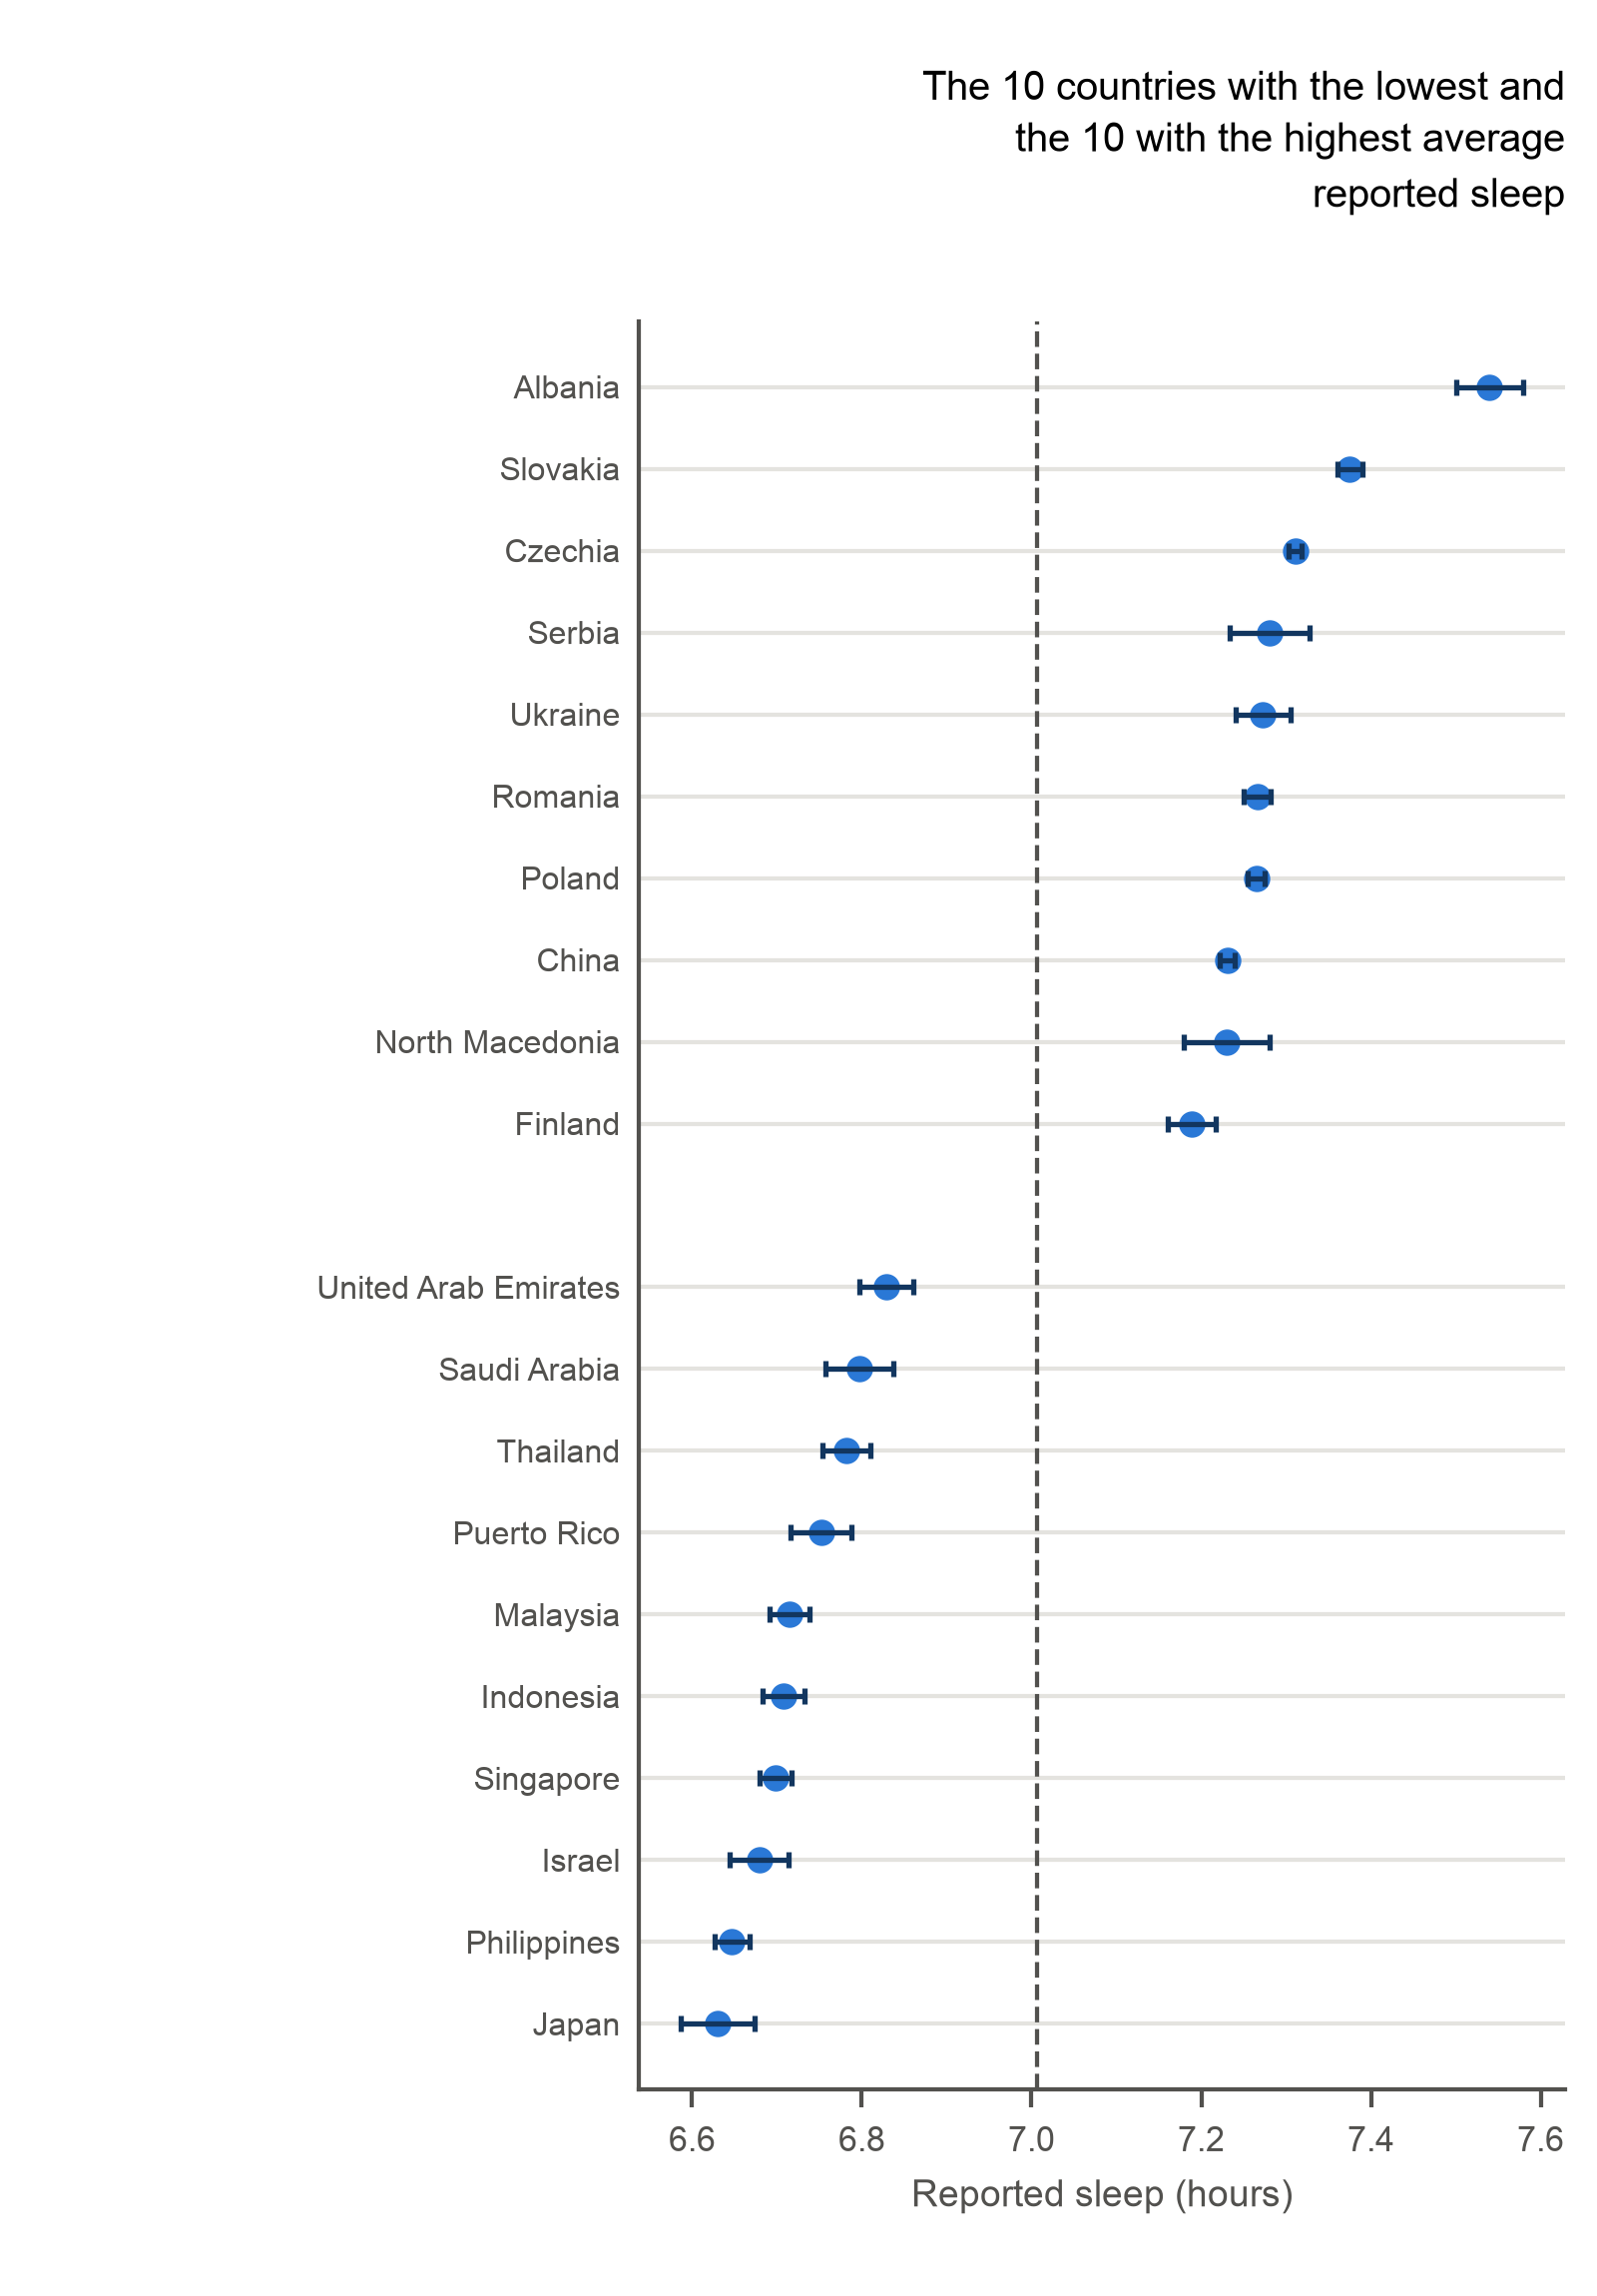
\includegraphics[width=\textwidth]{figures/report_fig_sleep_by_country_py.png}
\end{minipage}\hspace{0.04\textwidth}
\begin{minipage}[c]{0.42\textwidth}
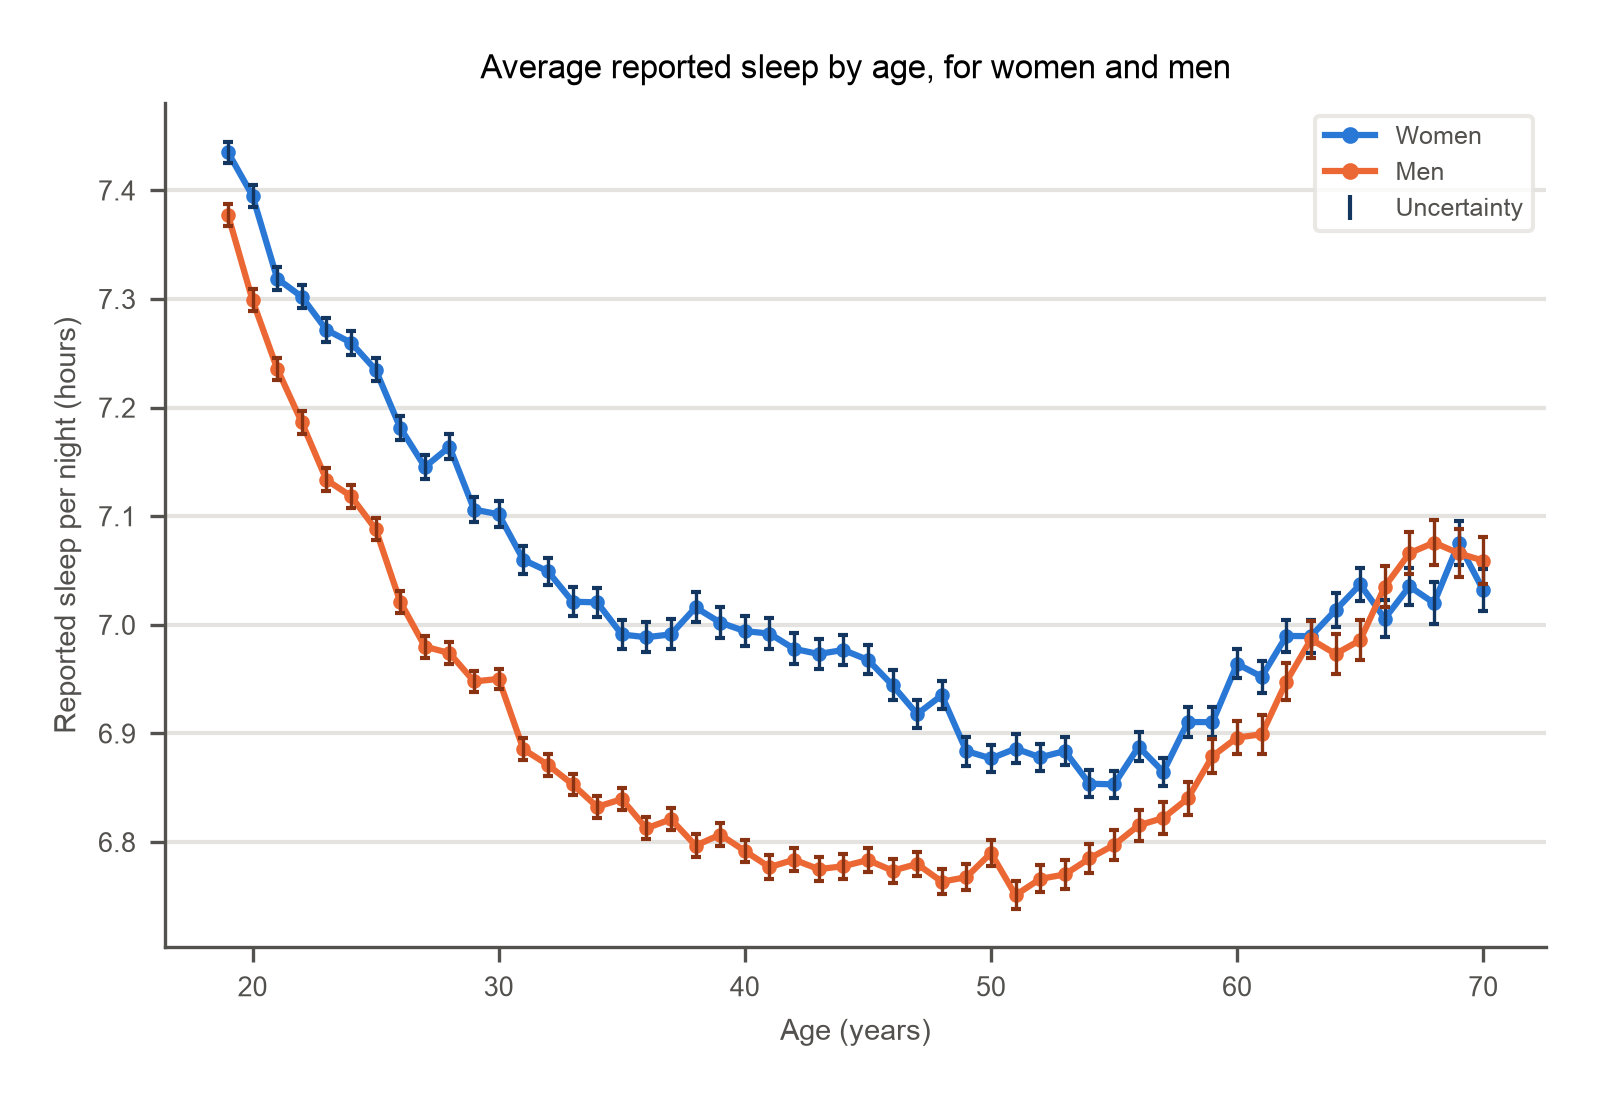
\includegraphics[width=\textwidth]{figures/report_fig_sleep_by_age_py.png}\\[0.2cm]
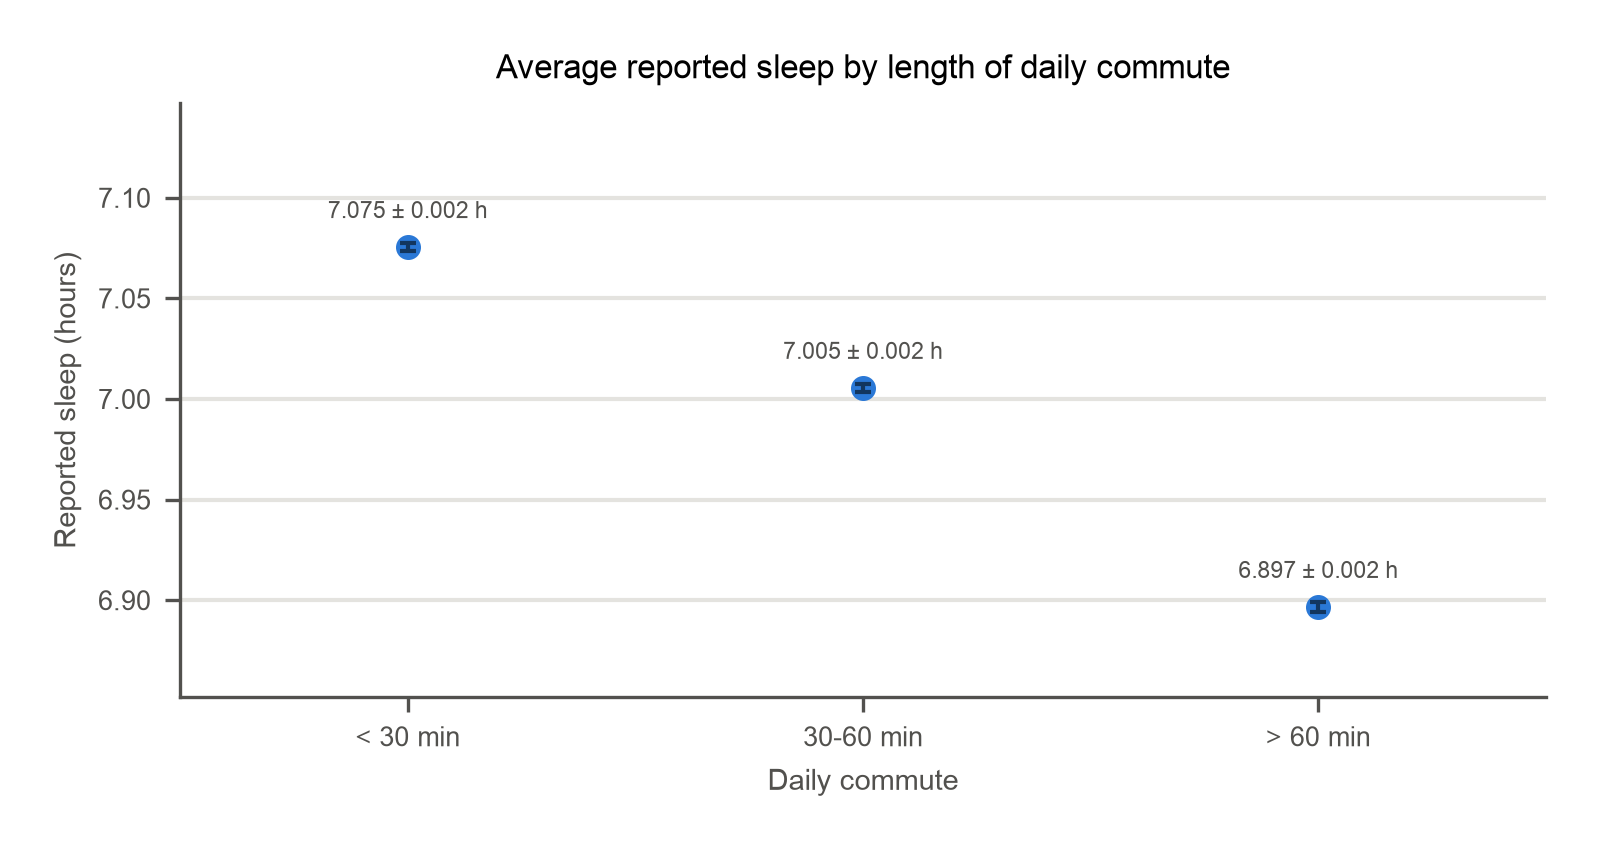
\includegraphics[width=\textwidth]{figures/report_fig_sleep_by_commute_py.png}
\end{minipage}
%if mean line in left panel is dotted changed dashed to dotted
\caption{Average reported sleep. Left: the 10 lowest and 10 highest of the 63 countries (dashed line is the average of all people). Top right: at every age, for women and men. Bottom right: by length of daily commute. Error bars show the statistical uncertainty.}
\label{fig:results}
\end{figure}

Women report $7.9 \pm 0.1$~minutes more sleep than men. Figure~\ref{fig:results} (top right) shows that sleep falls steeply from 7.41~hours at age 19 to 6.83~hours at age 50 and rises again afterwards to 7.04~hours at age 70, in agreement with the three phases reported by Coutrot et al.~\cite{coutrot}. The largest gap between the four 13-year age groups is $20.6 \pm 0.2$~minutes, between ages 19--31 and 45--57. The difference between women and men is largest between ages 35 and 45 (10 to 13 minutes) and almost disappears in the sixties. This may be related to retirement, but the data contains no information on employment. Finally, people who commute more than an hour report $10.7 \pm 0.2$~minutes less sleep than people who commute less than 30~minutes (Figure~\ref{fig:results}, bottom right). All differences are highly significant, but their effect sizes differ (Table~\ref{tab:groups}). Only the country difference is large ($g = 0.61$ to $0.79$); the age, commute and sex differences are small ($g = 0.32$, $g = 0.17$ and $0.12$). The multiple regression confirms the results but changes two of them. The commute difference grows from 10.7 to $14.1 \pm 0.2$~minutes, because long commuters are more common in countries where people sleep more, which partly hid the effect. The country differences shrink to 41 to 53 minutes, because Albania's respondents are young (76\% are aged 19--31) and young people sleep the most. Together, the four variables explain only 4.4\% of the variation in reported sleep between people. 

\begin{table}[!ht]
\centering
\small
\setlength{\tabcolsep}{4pt}
\begin{tabular}{llccccc}
\toprule
 & & \multicolumn{3}{c}{All countries together} & 
\multicolumn{2}{c}{Inside each country} \\
Comparison & Groups & Difference (min) & Significance & Hedges' $g$ & Same direction & Median (min) \\
\midrule 
Country & Albania vs.\ 9 lowest & 45 to 55 & $\geq 13\sigma$ & 0.61--0.79 & -- & -- \\ 
Age & 19--31 vs.\ 45--57 & $20.6 \pm 0.2$ & $106\sigma$ & 0.32 & 59 of 63 & 16.5 \\
Commute & $<30$ min vs.\ $>60$ min & $10.7 \pm 0.2$ & $56\sigma$ & 0.17 & 61 of 63 & 13.2 \\
Sex & women vs.\ men & $7.9 \pm 0.1$ & $53\sigma$ & 0.12 & 58 of 63 & 9.1 \\
\midrule
\multicolumn{7}{l}{Multiple regression: country 41 to 53, age $19.7 \pm 0.2$, commute $14.1 \pm 0.2$, sex $7.3 \pm 0.1$~minutes} \\
\bottomrule
\end{tabular}
\caption{Differences in average reported sleep between groups.} 
\label{tab:groups}
\end{table}

\textbf{Conclusion.} Among these respondents, the least sleep is reported in Japan and eight other countries that cannot be statistically separated from it, and the most in Albania, 45 to 55 minutes more. Men, people aged 45-57 and people commuting over an hour report the least sleep, both inside almost every country and in the regression. All differences are highly significant ($13\sigma$ or more) because the sample is very large, but only the country differences are large ($g \approx 0.6$ to $0.8$); the others are small compared with the spread of 1.06~hours between individuals. These results have limitations: the uncertainties are statistical only, sleep is self-reported in whole hours, the players of a mobile game are not a random sample, and the differences are correlations, not causes. 

\footnotesize
\setlength{\bibsep}{0pt}
\begin{thebibliography}{9}
\raggedright
\bibitem{watson} N.~F.~Watson \textit{et al.}, ``Recommended amount of sleep for a healthy adult: a joint consensus statement of the American Academy of Sleep Medicine and Sleep Research Society'', \textit{Sleep} \textbf{38}, 843--844 (2015). 
\bibitem{coutrot} A.~Coutrot \textit{et al.}, ``Reported sleep duration reveals segmentation of the adult life-course into three phases'',  
\textit{Nature Communications} \textbf{13}, 7697 (2022).
Data: \url{https://osf.io/j7sd4/?view_only=92c1aa56abfc4d0f99501c9f260fa324}
(accessed September 16, 2026).
\end{thebibliography} 

\end{document} 
